
We perform a reweighting to take into account the difference 
between the pile-up model used to generate the simulated data samples.
Because the expected pile-up distribution depends on the instantaneous 
luminosity, we reweight to the target distribution that corresponds to 
the dataset used.
The result of applying this procedure to the EPS, post-EPS and LP datasets
is shown in Figures \ref{subfig:lp_pureweight_eps}, \ref{subfig:lp_pureweight_posteps}
and \ref{subfig:lp_pureweight_lp} respectively. 
In all cases we find good agreement between the data and the simulation
after reweighting.

\begin{figure}[!hbtp]
\centering
\subfigure[]{
\centering
\label{subfig:lp_pureweight_eps}
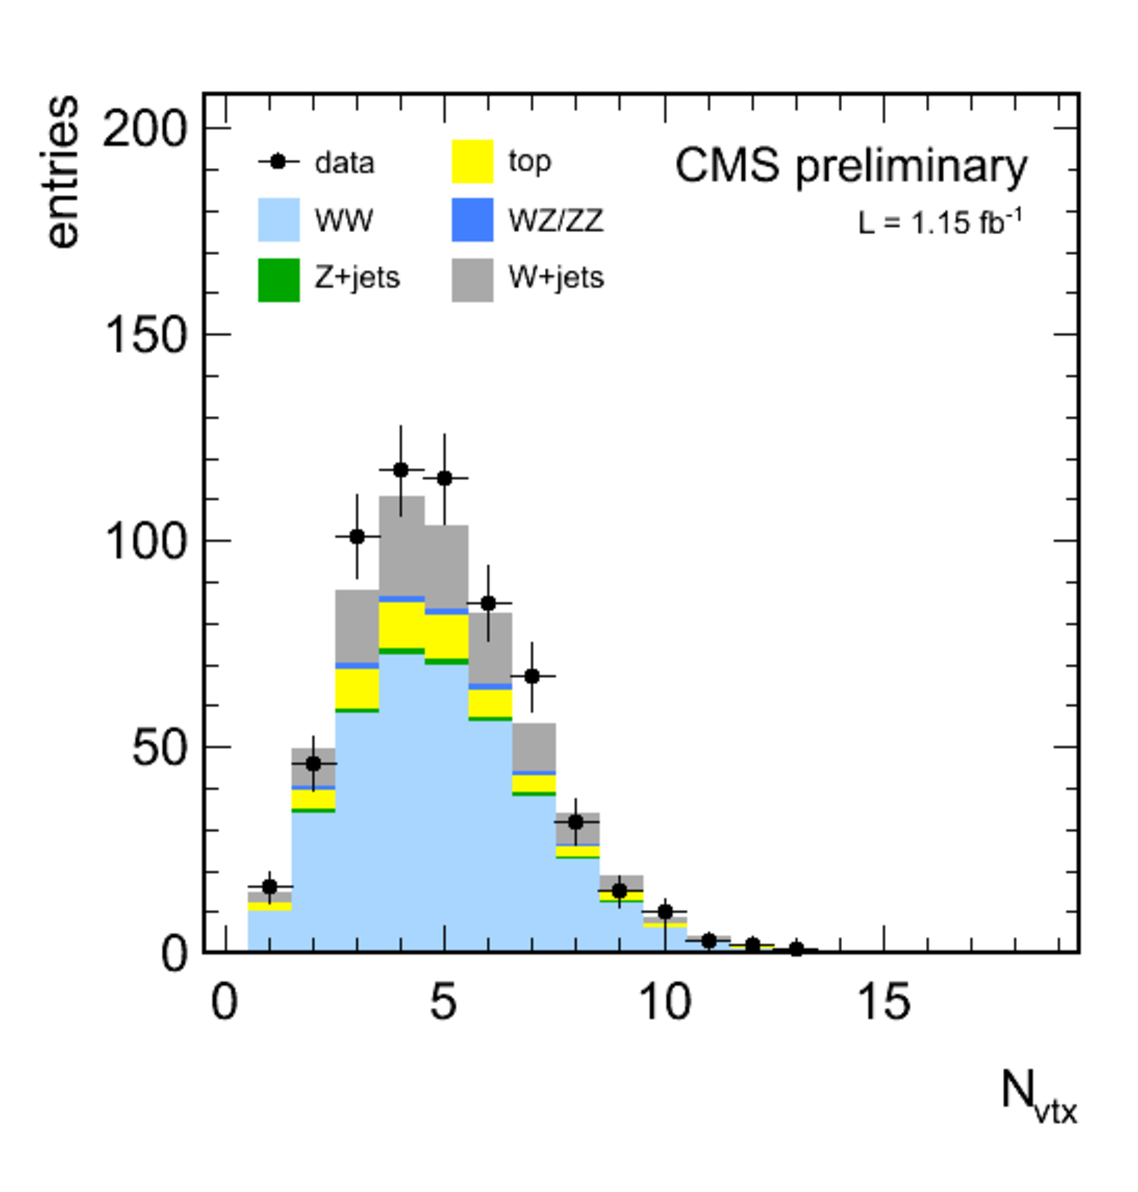
\includegraphics[width=.4\textwidth]{lp_figures/puReweight/histo_nvtx_ww0j_allhwwcuts_EPS.pdf}}
\subfigure[]{
\centering
\label{subfig:lp_pureweight_posteps}
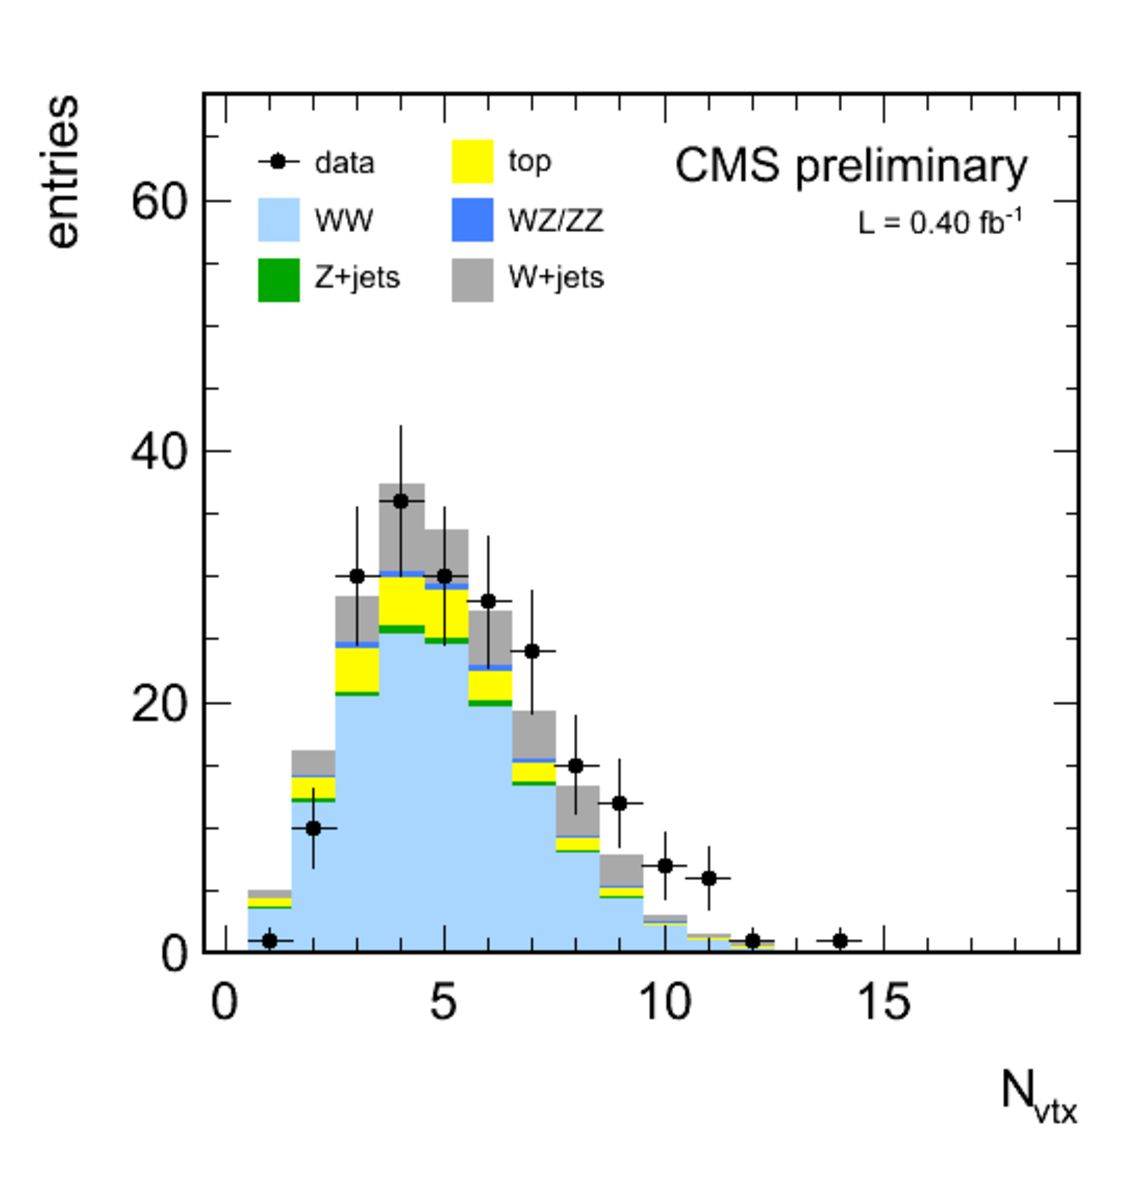
\includegraphics[width=.4\textwidth]{lp_figures/puReweight/histo_nvtx_ww0j_allhwwcuts_POSTEPS.pdf}}\\
\subfigure[]{
\centering
\label{subfig:lp_pureweight_lp}
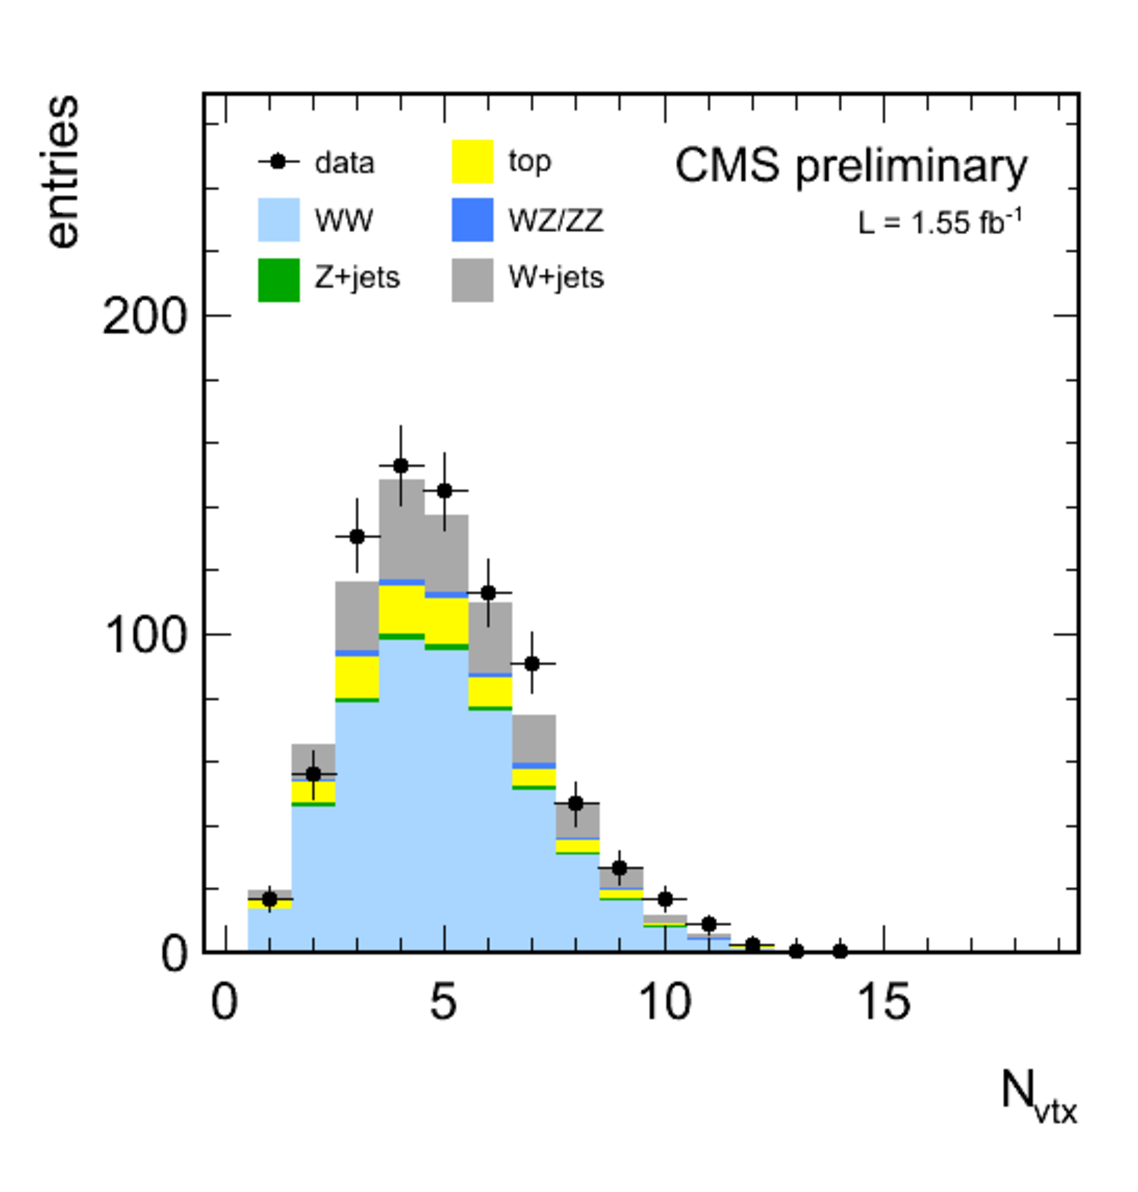
\includegraphics[width=.4\textwidth]{lp_figures/puReweight/histo_nvtx_ww0j_allhwwcuts.pdf}}
\caption{The number of reconstructed vertices in data and simulation 
at the WW preselection level after pile-up reweighting
according to the expected pile-up multiplicity
\subref{subfig:lp_pureweight_eps} in the EPS dataset;
\subref{subfig:lp_pureweight_posteps} in the post-EPS dataset;
\subref{subfig:lp_pureweight_lp} in the LP dataset;
}
\label{fig:lp_ww0j_dilep}
\end{figure}

